\cleardoublepage

\chapter{Instalación y puesta en marcha}
\label{makereference7}

Para poner en funcionamiento el proyecto deberemos tener todos lo elementos que lo componen:
\begin{itemize}
\item Nodo.
\item Servidor de datos.
\item Servidor de cálculo. Puede estar alojado en la misma máquina que el servidor de datos.
\item Sistema de visualización. En este caso, estar registrado en ThingSpeak y tener una clave de aplicación.
\end{itemize}

\section{Nodo}
\label{makereference7.1}
\subsection{Requisitos}
\label{makereference7.1.2}
	\begin{itemize}
		\item \textbf{Raspberry Pi 3 model B} con una distribución Linux (\href{https://www.raspberrypi.org/downloads/raspbian/}{Raspbian}).
		\item Conexión a Internet.
		\item \href{https://www.adafruit.com/product/385}{Sensor DHT22}.
		\item Conversor analógico-digital \href{https://www.adafruit.com/product/856}{MCP3008}.
		\item Piranómetro \href{https://www.apogeeinstruments.co.uk/content/SP-212-215-manual.pdf}{SP-212}.
		\item SPI activo en la Raspberry con ``raspi-config''.
	\end{itemize}

El cableado de los componentes HW está descrito en la figura \ref{wiring}.
\begin{figure}[htb]
	\begin{center}
		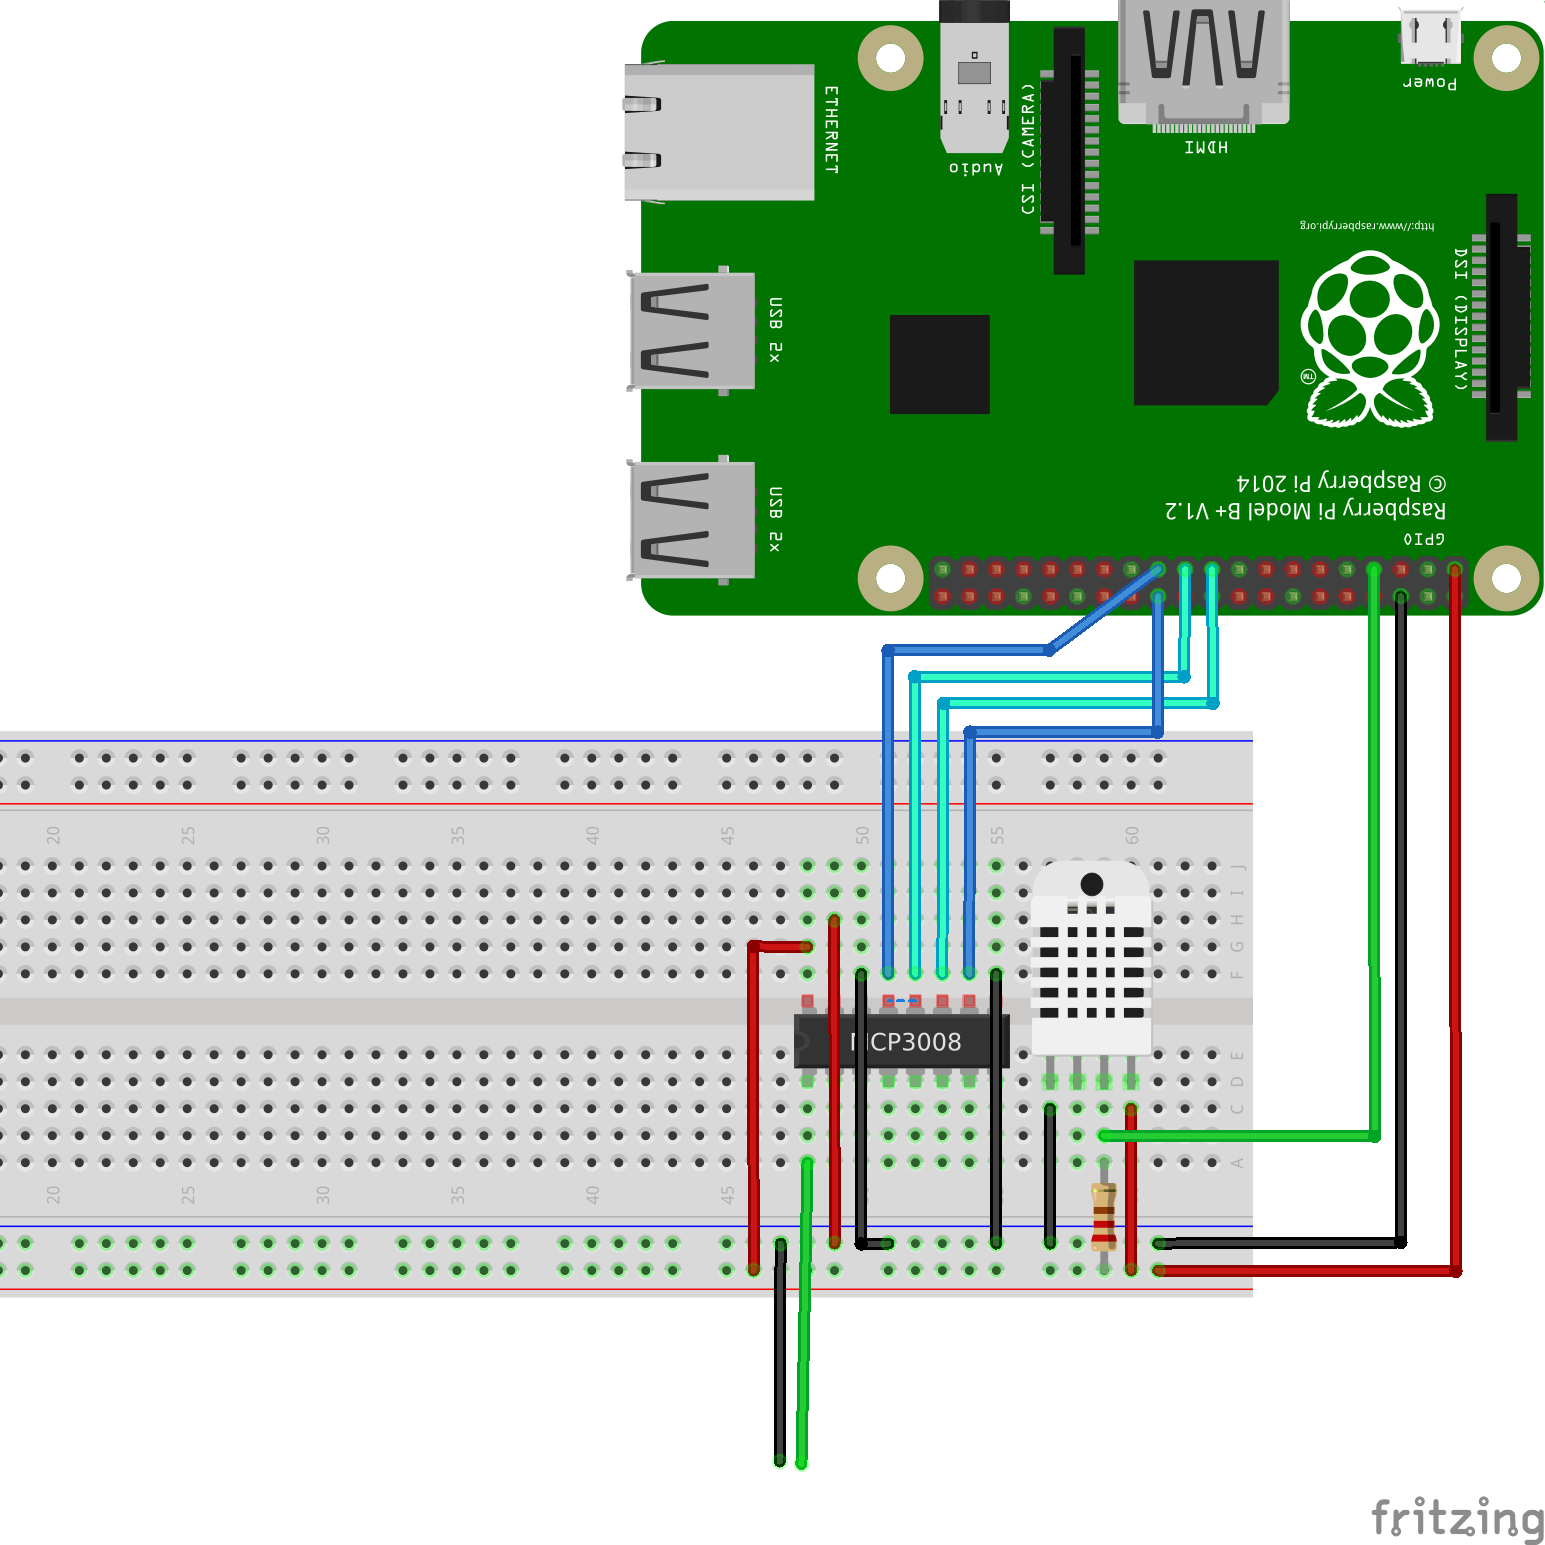
\includegraphics[width=12cm]{figures/solar_project_node_diagram.png}
		\caption{Cableado del nodo}
	\end{center}

Por defecto, Ubuntu arranca el servicio después de instalarlo. Si la distribución Lunix sobre la cual se instala no realiza esta acción por defecto, se deberá configurar debidamente para arrancarlo.

En este proyecto se utiliza la configuración por defecto de Mosquitto. Para más información sobre su configuración, consultar \href{https://www.digitalocean.com/community/tutorials/how-to-install-and-secure-the-mosquitto-mqtt-messaging-broker-on-ubuntu-16-04}{más información}.

	\label{wiring}
\end{figure}

\subsection{Ficheros}
\label{makereference7.1.3}
Los archivos necesarios para la instalación del software del nodo se encuentran disponibles en \href{https://github.com/MrSlide22/TFG/node}{Github}.

\begin{itemize}
	\item Introduce el directorio \textbf{node} en tu Rapsberry Pi
	\item Cambia las variables \textbf{brokerIp, brokerPort, topic, ubication} en solar\_node.py
\end{itemize}

\subsection{Dependencias}
\label{makereference7.1.4}
	\begin{itemize}
		\item Actualizar
\lstset{language=bash}
\begin{lstlisting}[frame=single]
$ sudo apt-get update
$ sudo apt-get upgrade
\end{lstlisting}
		\item Python 2.7 (\cite{ARP:Python:2017})
\begin{lstlisting}[frame=single]
$ sudo apt-get install python2.7 build-essential 
python-pip python-dev
\end{lstlisting}
		\item Paho (\cite{ARP:Paho:2017})
\begin{lstlisting}[frame=single]
$ pip install paho-mqtt
\end{lstlisting}
		\item WiringPi (\cite{ARP:Wiring:2017})
\begin{lstlisting}[frame=single]
$ pip install wiringpi2
\end{lstlisting}
		\item Adafruit\_DHT (\cite{ARP:Adafruit:2017})
\begin{lstlisting}[frame=single]
$ git clone 
https://github.com/adafruit/Adafruit_Python_DHT.git
$ cd Adafruit_Python_DHT
$ sudo python setup.py install
\end{lstlisting}
		\item Adafruit\_GPIO
\begin{lstlisting}[frame=single]
$ git clone 
https://github.com/adafruit/Adafruit_Python_GPIO.git
$ cd Adafruit_Python_GPIO
$ sudo python setup.py install
\end{lstlisting}
		\item Adafruit\_MCP3008
\begin{lstlisting}[frame=single]
$ git clone 
https://github.com/adafruit/Adafruit_Python_MCP3008.git
$ cd Adafruit_Python_MCP3008
$ sudo python setup.py install
\end{lstlisting}
	\end{itemize}

\subsection{Puesta en marcha del nodo}
\label{makereference7.1.5}
Para arrancar el nodo se deberá haber seguido todos los pasos anteriores. Posteriormente, desde un terminal de la Raspberry, ir a la carpeta donde se han guardado el código fuente y ejecutar el comando: 

\lstset{language=bash}
\begin{lstlisting}[frame=single]
$ sudo python solar_node.py
\end{lstlisting}

Se debe ser superusuario para poder ejecutar este comando.

% TODO - referenciar "descripción del nodo" de la línea de abajo
Para obtener más información sobre cómo utilizar el nodo ver Descripción del nodo o ejecutar:

\lstset{language=bash}
\begin{lstlisting}[frame=single]
$ sudo python solar_node.py -h
\end{lstlisting}

\section{Servidor de datos}
\label{makereference7.2}
\subsection{Requisitos previos}
\label{makereference7.3}
\begin{itemize}
\item Máquina con distribucion Linux instalada. Recomendable Debian, Fedora, OpenSUSE o Ubuntu.
\item conexión a internet.
\item IP fija y opcionalmente, nombre de dominio.
\end{itemize}

La instalación de un broker MQTT es muy sencilla (una de sus principales ventajas). Para ello basta con instalar el demonio mosquitto a través del siguiente comando:

Ejemplo de instalación en Ubuntu:
\lstset{language=bash}
\begin{lstlisting}[frame=single]
$ sudo apt-get install mosquitto
\end{lstlisting}

Por defecto, Ubuntu arranca el servicio después de instalarlo. Si la distribución Lunix sobre la cual se instala no realiza esta acción por defecto, se deberá configurar debidamente para arrancarlo.

En este proyecto se utiliza la configuración por defecto de Mosquitto. Para más información sobre su configuración, consultar \href{https://www.digitalocean.com/community/tutorials/how-to-install-and-secure-the-mosquitto-mqtt-messaging-broker-on-ubuntu-16-04}{más información}.

\section{Servidor de cálculo}
\label{makereference7.3}

\subsection{Requisitos previos}
\label{makereference7.3.1}

\begin{itemize}
\item Máquina con distribución Linux.
\item Python 2.7.
\item Conexión a internet.
\item IP fija y opcionalmente, nombre de dominio.
\end{itemize}

\subsection{Instalación}
\label{makereference7.3.2}
Los archivos necesarios para la instalación del software del servidor de cálculo se encuentran disponibles en \href{https://github.com/MrSlide22/TFG/server}{Github}.

\begin{itemize}
	\item Introduce el directorio \textbf{server} en el servidor.
	% TODO - revisar cuales son las variables necesarias
	\item Cambia las variables \textbf{ThingSpeakKey} en solar\_server.py
\end{itemize}